This chapter explains some of the fundamental concepts used in the development in this thesis.
In section \ref{sec:concept-cancer} the concept of cancer is introduced. The characteristics of cancerous cells compared to normal cells, the molecular mechanisms responsible for their onset and those that facilitate their maintenance and proliferation.
In section \ref{sec:concept-alteration} the genetic and epigenetic changes in cancer cells are detailed.
In section \ref{sec:concept-data} the clinical, genetic and epigenetic data publicly available used for cancer data analysis are described. Their computational representation and data structures available to manipulate large collections of data are detailed.
Finally, in section \ref{sec:concept-analysis} several techniques of data analysis
used to extract biological knowledge from this data are presented.


\section{Cancer} \label{sec:concept-cancer}

Tumors are complex tissues composed of multiple distinct cell types that participate in heterotypic interactions with one another. For the onset of tumorigenesis,  cancer cells create a "tumor microenvironment"
 recruiting normal cells which are active participants in tumorigenesis rather than passive bystanders.
If compared to normal cells, cancer cells acquired capabilities which includes sustaining proliferative signaling,
 evading growth suppressors, resisting cell death, enabling replicative immortality,
 inducing angiogenesis, activating invasion and metastasis, reprogramming of energy metabolism and
 evading immune destruction \cite{hanahan2011hallmarks}.  Some examples of these acquired capabilities are described below.

\begin{description}
  \item [Sustaining Proliferative Signaling]
  While normal tissues carefully control the production and release of growth-promoting
  signals the cancer cells deregulate these signals in ways that promote proliferation.
    Cancer cells can acquire the capability to sustain proliferative signaling in a number of alternative ways: They may produce growth factor ligands themselves, they may send signals to stimulate normal cells within the supporting tumor-associated stroma, to supply them with various growth factors \cite{cheng2008transforming}, or
   they may elevate the levels of receptor proteins displayed on the cancer cell surface,
   rendering such cells hyperresponsive to otherwise-limiting amounts of growth factor ligand.
   Cancer cell also disrupts Negative-Feedback Mechanisms that Attenuate Proliferative Signaling,
   for example,  loss-of-function mutations or promoter methylation of the \sigla{PTEN}{Phosphatase and tensin homolog}, a tumor suppressor, amplify \sigla{PI3K}{Phosphatidylinositol 3-kinase} signaling and promote tumorigenesis in a variety of experimental models of cancer \cite{jiang2009pi3k}. A second example is the oncogene \sigla{RAS}{Rat Sarcoma}, some mutations affecting it compromise Ras GTPase activity,  a protein that normally regulates the inactivation of Ras. In addition to the oncogenic mutations in Ras, another mechanism affecting this gene showed silence of the regulatory Ras GTPase proteins through CpG methylation \cite{jin2007epigenetic}.
   \item [Evading growth suppressors]  Cancer cells must also circumvent actions of tumor suppressor genes that negatively regulate cell proliferation. One example of tumor suppressor proteins is the  \sigla{RB}{retinoblastoma-associated},
   that integrates signals from diverse extracellular and intracellular sources and, in response, decides whether or not a cell should proceed through its growth-and-division cycle \cite{burkhart2008cellular}.
   Cancer cells with defects in RB pathway function are thus missing the services of a critical gatekeeper of cell-cycle progression whose absence permits persistent cell proliferation. Another example is the TP53 proteins that
    receives inputs from stress and abnormality sensors that function within the cell's intracellular operating systems.
    This protein can activate apoptosis if it received a signal of irreparable damage to the cellular subsystems, or it can
    interrupt the cell-cycle progression if it receives signals that the degree of damage to the genome is excessive, or if the levels of nucleotide pools, growth-promoting signals, glucose, or oxygenation are suboptimal \cite{hanahan2011hallmarks}.
    Moreover, disruption of such self-attenuating
    signaling may contribute to the development of
    adaptive resistance toward drugs targeting mitogenic signaling.
    To evade those growth suppressors proteins tumor cells developed mechanisms of contact inhibition and its evasion.

    \item[Resisting Cell Death]
    The loss of TP53 tumor suppressor function, which eliminates this critical damage sensor from the apoptosis-inducing circuitry, is a strategy of tumor cells to limit or circumvent apoptosis \cite{hanahan2011hallmarks}.
\end{description}

Those capabilities, which enable tumor growth and metastatic dissemination, were acquired mainly due to a genetic diversity
 generated  by genome instability \cite{hanahan2011hallmarks}.
 A multistep tumor progression can be portrayed as
a succession of clonal expansions, which can be triggered by non mutational changes (epigenetic mechanisms such as DNA methylation and histone modifications \cite{berdasco2010aberrant})
or mutational changes affecting the regulation of gene expression.

To increase  the rates of mutation, cancer cells often breakdown components of the genomic maintenance machinery
that normally monitor genomic integrity and force genetically damaged cells into either senescence or apoptosis \cite{jackson2009dna}, more specifically those involved in detecting DNA damage and activating the repair machinery, in directly repairing damaged DNA, and in inactivating or intercepting mutagenic molecules before they have damaged the DNA \cite{negrini2010genomic}. Another major source of tumor-associated genomic instability is the loss of telomeric DNA  in many tumors that generates karyotypic instability and associated amplification and deletion of chromosomal segments \cite{artandi2009telomeres}.  Recurrence  of these amplifications and deletions aberrations at particular sites in the genome
indicates that they are likely to harbor genes whose alteration favors neoplastic progression \cite{korkola2010breast}.


\section{Genetics and epigenetics alterations} \label{sec:concept-alteration}

While genetics is the study of heritable changes in gene activity or function due
to the direct alteration of the DNA sequence such as point mutations, deletions,
insertions, and translocation, epigenetics is the study of  those not associated with any change of the DNA sequence \cite{moore2013dna}.
Even though all cells in an organism contain the same genetic information,
this epigenetic mechanism controls which gene are expressed enabling the existence of
a diversified gene expression profiles
in a variety of cells and tissues in multicellular organisms.


\subsection{DNA methylation}
DNA methylation is an epigenetic mechanism involving the transfer of a methyl group to the C5
position of the cytosine to form 5-methylcytosine, which regulates
gene expression  by either blocking the binding of Transcription factors or
recruiting proteins involved in gene repression \cite{moore2013dna}.
The pattern of DNA methylation in the genome can change by DNA methylation and demethylation process,
these processes are involved in cell differentiation as unique DNA methylation pattern is able to regulate
tissue-specific gene transcription \cite{moore2013dna}.

The DNA methylation process is mediated by the family of \sigla{Dnmts}{DNA methyltransferases}
proteins which catalyze the transfer of a methyl group from \sigla{SAM}{S-adenyl methionine} to the fifth carbon of cytosine residue to form \sigla{5mc}{5-methylcytosine}.
The main proteins responsible for this transfer are the Dnmt3a and Dnmt3b, which
are involved in establishing a new methylation pattern to unmodified DNA, and Dnmt1, which is responsible
to the methylation of a daughter strand during the DNA replication process.

The majority of DNA methylation occurs on cytosines that precede a guanine nucleotide (CpG sites), however
\citeonline{xie2012base} it has already been reported a significant percentage of methylated non-CpG sites \cite{xie2012base}.

The role of DNA methylation varies in different genomic regions.
Within intergenic regions, the DNA methylation represses the expression of potentially harmful genetic elements,
while within promoter regions containing CpG islands, stretches of DNA roughly 1000 base pairs long that have a higher CpG density than the rest of the genome and  often  are not methylated  \cite{bird1985fraction}, results in stable silencing of gene expression \cite{mohn2008lineage}.
Also, within the gene body, region of the gene past the first exon, the methylation of the first exon leads to gene silencing
\cite{brenet2011dna}.

% Falar sobre regioes distais ? Enhancers ?

\subsection{Histone modifications}

This process of transcription regulation involving DNA methylation,
works in association with histone modifications and noncoding RNAs.

Normally, the DNA is wrapped around the histone proteins forming small, packaged sections called nucleosomes.
This association is capable of inhibiting gene expression since a more compact region
hinders the accessibility of transcription factors.

Those histones might have chemical modifications (methylation, acetylation, ubiquitination, and phosphorylation) added to three specific amino acids on their N-terminal tail which influences how DNA strands are packaged and their transcriptional activity.
Those modifications that loosen DNA association with histones generally provide a permissive environment for transcription, whereas the ones that tights them repress gene expression \cite{moore2013dna}.

These modifications involved in adding and/or stripping histone markers in order to impose a repressive state on a gene region, are lead by histone-modifying enzymes and are in general in cooperation with the Dnmts proteins
which are involved in the mechanism of DNA methylation.
For example, Dnmt1 and Dnmt3 are known to bind to the histone methyltransferase SUV39H1 that
restricts gene expression by methylation on \sigla{H3K9}{histone H3 lysine 9} \cite{fuks2003dna}.
Other examples are Dnmt1 and Dnmt3b than can both bind to histone deacetylases that remove
acetylation from histones to make DNA pack more tightly and restrict access for transcription \cite{fuks2000dna,geiman2004dnmt3b}.
Also, \sigla{H3K36}{histone H3 lysine 9} trimethylation, a repressive histone mark, stimulates the methyltransferase activity, the \sigla{H3K4me3}{H3K4 trimethylation} prevents it \cite{ooi2007dnmt3l,zhang2010chromatin}.

The miRNAs have emerged as another important epigenetic mechanism that influences gene expression.
It can repress gene expression by inhibiting translation or inducing RNA degradation \cite{berezikov2011evolution} and
 it not only can regulate histone modifications and Dnmt expression thus regulating DNA methylation \cite{benetti2008mammalian,sinkkonen2008micrornas}, but also the DNA methylation can regulate the expression of miRNAs \cite{han2007dna,lujambio2008microrna}.

Overall, miRNAs, DNA methylation, and histone modifications work closely
together to regulate gene expression \cite{moore2013dna}.

% Tabela de modificacoes de histona ?

\subsection{Genetics alterations}

Although the haploid human genome consists of 3 billion nucleotides,
changes in even a single base pair might result in dramatic physiological malfunctions.
A mutation, defined as any alteration in the DNA sequence,
can be a  germ-line mutation, which occurs in a germ-line cell
(one that will give rise to gametes) and
can be passed to a descendant of the organism, and somatic mutations,
which occurs in a somatic cell (one that develops into the body tissues) and
are never transmit to their descendants \cite{clancy2008genetic}.


 A single base pair alteration that is present in at least 1\% of the population
is called  \sigla{SNP}{single nucleotide polymorphism} and is generally used to refer to a
normal variation (does not directly cause disease) \cite{clancy2008genetic}.

An example of a point mutations that is able to alter proteins is the insertion or the deletion of a single base, called frameshift mutations. This change of nucleotides alters the codons (a group of three nucleotides) read by the ribosomes, which
 affects the protein resulted during the translation process. Table \ref{mutation-effect}
 show a classification of translational effect of variant allele \cite{GTAK_maf,maf}.

\begin{landscape}

% Please add the following required packages to your document preamble:
% \usepackage{booktabs}
\begin{table}[]
\centering
\caption[Translational effect of variant allele]{Translational effect of variant allele. \cite{GTAK_maf}}
\label{mutation-effect}
\begin{tabular}{@{}ll@{}}
\toprule
\toprule
\multicolumn{1}{c}{\textbf{Variant\_Classification}} & \multicolumn{1}{c}{\textbf{Group}} \\ \midrule \midrule
Frame\_Shift\_Del & Deletion that moves the coding sequence out of frame \\
Frame\_Shift\_Ins & Insertion that moves the coding sequence out of frame \\
Missense\_Mutation &  The point mutation alters the protein structure by one amino acid \\
Nonsense\_Mutation & A premature stop codon is created by the variant \\
Silent & Variant is in coding region of the chosen transcript, but protein structure is identical \\
Splice\_Site & The variant is within two bases of a splice site.  \\
In\_Frame\_Del & Deletion that keeps the sequence in frame \\
In\_Frame\_Ins & Insertion that keeps the sequence in frame \\
Translation\_Start\_Site & Point mutation, insertion or deletion that overlaps the start codon \\
Nonstop\_Mutation & variant removes stop codon. \\
3'UTR & The variant is on the 3'UTR for the chosen transcript \\
3'Flank & The variant is downstream of the chosen transcript (within 3kb) \\
5'UTR & The variant is on the 5'UTR for the chosen transcript \\
5'Flank & The variant is upstream of the chosen transcript (within 3kb) \\
IGR & Intergenic region. Does not overlap any transcript. \\
Intron & The variant lies between exons within the bounds of the chosen transcript. \\
De\_novo\_Start\_InFrame & New start codon is created in frame relative to the coded protein. \\
De\_novo\_Start\_OutOfFrame & New start codon is created out of frame relative to the coded protein. \\
RNA & The variant lies on one of the RNA transcripts. \\
lincRNA & The variant lies on one of the lincRNAs. \\\bottomrule
\end{tabular}
\end{table}

\end{landscape}
Not only changes in DNA can occur on a single nucleotide called point mutations but they can
also occur at the level of the chromosome, in which large segments of chromosomes are altered
(deleted, duplicated, inverted, translocated to different chromosomes, rearranged)
resulting in levels of gene expression, the complete absence of genes, or the alteration of gene sequence.
\citeonline{feuk2006structural} define structural variants as genomic alterations that involve segments
of DNA that are larger than $1 kb$ which can be microscopic ($> 3Mb$) or submicroscopic ($1 kb$ to $3 Mb$) variants,
and also define smaller ($<1 kb$) variations or polymorphisms that involve the copy-number change
 of a segment of DNA as insertions or deletions (indels).
A type of structural variant is the \sigla{CNV}{copy number variation} which refers to a segment of DNA that is $1 kb$ or larger and is present at a variable copy number in comparison with a reference genome, while \sigla{CNP}{Copy-number polymorphism} are CNVs that occurs in more than 1\% of the population. Also, it is common to refer to changes in copy number that have arisen in somatic tissue as copy number alterations/aberrations (CNAs or SCNAs) and changes in copy number in germline cells
 as copy number variations (CNVs).
Table \ref{mutation} summarizes the types of mutations.


% The size of CNVs ranges from 50bp to 3 Mb \cite{macdonald2013database}

% Within this class, \sigla{CNV}{copy number variation}, which involves unbalanced rearrangements
% that increase or decrease the DNA content, accounts for the largest component by far9,11.
% We now typically define the size of CNVs as larger than 50 bp12, whereas smaller elements are known as insertions
% or deletions (indels). These structural variations encompass more polymorphic base pairs than SNPs by an order of magnitude

 \begin{landscape}
 \bgroup
 \def\arraystretch{2.0}%  1 is the default, change whatever you need

 % Please add the following required packages to your document preamble:
 % \usepackage{multirow}
 \begin{table}[]
 \centering
 \small
 \caption[Types of DNA Mutations and Their Impact]{Types of DNA Mutations and Their Impact \cite{comis_cnv,clancy2008genetic,feuk2006structural}}
 \label{mutation}
 \begin{tabular}{p{4cm}c|p{13cm}}
 \hline \hline
 \multicolumn{1}{c}{\textbf{Class of Mutation}} & \multicolumn{1}{c}{\textbf{Type of Mutation}} & \multicolumn{1}{c}{\textbf{Description}}  \\ \hline \hline
\multicolumn{1}{c|}{\multirow{3}{*}{\parbox{3cm}{\vspace{1.2cm} Point mutation}}}
& Substitution  & One base is incorrectly added during replication and replaces the pair in the corresponding position on the complementary strand \\  \cline{2-3}
\multicolumn{1}{c|}{}                                       & Insertion                                     & One or more extra nucleotides are inserted into replicating DNA, often resulting in a frameshift                                 \\  \cline{2-3}
\multicolumn{1}{c|}{}                                       & Deletion                                      & One or more nucleotides is "skipped" during replication or otherwise excised, often resulting in a frameshift                  \\ \hline
\multicolumn{1}{c|}{\multirow{4}{*}{\parbox{4cm}{\vspace{1.2cm} Chromosomal mutation}}}  &
Inversion  & A segment of DNA that is reversed in orientation with respect to the rest of the chromosome. \\  \cline{2-3}
\multicolumn{1}{l|}{}    & Deletion & A region of a chromosome is lost,
resulting in the absence of all the genes in that area      \\  \cline{2-3}
\multicolumn{1}{l|}{}    & Duplication   or low-copy repeat   & A segment of DNA $<1 kb$ in size that occurs in two or more copies per haploid genome, with the different copies sharing $>90\%$ sequence identity.  \\  \cline{2-3}
\multicolumn{1}{l|}{}    & Translocation   &  A change in position of a chromosomal segment within a genome that involves no change to the total DNA content. Translocations can be intra- or inter- chromosomal.   \\ \hline
\multicolumn{1}{l|}{\multirow{2}{*}{Copy number variation}} & Gain/Amplification
 & A single-copy gain or a multi-copy amplification of the entire gene  \\  \cline{2-3}
\multicolumn{1}{l|}{}  & Loss/Deletion  &
A loss  for part or all of a coding region within the gene footprint in a single allele/copy (hemizygous deletion) or deletion  for part or all of a coding region within the gene footprint in both alleles/copies (homozygous deletion). \cite{comis_cnv} \\\hline
\end{tabular}
 \end{table}
 \egroup
 \end{landscape}

 \section{Databases and data structure} \label{sec:concept-data}

 Recent technological developments allowed the deposition of large amounts of genomic and epigenomic data, such as gene expression, DNA methylation, and genomic localization of transcription factors, into freely available public international consortia like The Cancer Genome Atlas (TCGA), The NCI's Genomic Data Commons (GDC), The Encyclopedia of DNA Elements (ENCODE), and The NIH Roadmap Epigenomics Mapping Consortium (Roadmap) \cite{Hawkins}.
 Subsection \ref{susec:db} presents an overview of those consortia and subsection  \ref{susec:structure} presents
 some of the computational data formats and data structures used to represent the biological data.

\subsection{Databases} \label{susec:db}
\begin{description}
  \item [The Cancer Genome Atlas (TCGA):] The TCGA consortium, which was a \sigla{NIH}{National Institute of Health} initiative, made publicly available molecular and clinical information for more than 30 types of human cancers including exome (variant analysis), single nucleotide polymorphism (SNP), DNA methylation, transcriptome (mRNA), microRNA (miRNA) and proteome. Sample types available at TCGA are primary solid tumors, recurrent solid tumors, blood-derived normal and tumor, metastatic, and solid tissue normal \cite{weinstein2013cancer}. This project was ended in mid-2016 and its data was moved to  the NCI Genomic Data Commons (GDC).
  \item [The Genomic Data Commons (GDC):]  The NCI's Genomic Data Commons (GDC) provides the cancer research community with a unified data repository that enables data sharing across cancer genomic studies in support of precision medicine.
  It supports numerous cancer genome programs at the NCI \sigla{CCG}{Center for Cancer Genomics}, including The Cancer Genome Atlas (TCGA) and Therapeutically Applicable Research to Generate Effective Treatments (TARGET) \cite{GDC_web}.
  Those data is harmonized against GRCh38 (hg38) using GDC Bioinformatics Pipelines which provides methods to the standardization of biospecimen and clinical data, the re-alignment of DNA and RNA sequence data against a common reference genome build GRCh38, and the generation of derived data. Also, this repository has a Legacy Archive to provide access to a unmodified copy of data that was previously stored in CGHub \cite{wilks2014cancer} and in the TCGA Data Portal hosted by the TCGA Data Coordinating Center (DCC), in which uses as references GRCh37 (hg19) and GRCh36 (hg18).
  \item [The Encyclopedia of DNA Elements (ENCODE):] Found in 2003 by the \sigla{NHGRI}{National Human Genome Research Institute}, the project aims to build a comprehensive list of functional elements that have an active role in the genome, including regulatory elements that govern gene expression. Biosamples include immortalized cell lines, tissues, primary cells and stem cells \cite{encode2011user}.
  \item [The NIH Roadmap Epigenomics Mapping Consortium:] This was launched with the goal of producing a public resource of human epigenomic data in order to analyze biology and disease-oriented research. Roadmap maps DNA methylation, histone modifications, chromatin accessibility, and small RNA transcripts in stem cells and primary ex vivo tissues
  \cite{Fingerman,Bernstein}.
\end{description}

 Briefly, these consortia provide large-scale epigenomic data onto a variety of microarrays and \sigla{NGS}{next-generation sequencing} platforms. Each consortium encompasses specific types of biological information on specific type of tissue or cell and, when analyzed together, it provides an invaluable opportunity for research laboratories to better understand the developmental progression of normal cells to cancer state at the molecular level and importantly, correlate these phenotypes with tissue of origins.

\subsection{Data and data structure} \label{susec:structure}

If previously the main bottleneck to scientific progress in cellular biology was data collection, now this
 bottleneck shifted to analysis of data \cite{mcpherson2009next}.
 The large-scale genomic data mining, which is the process of using many diverse datasets to address a specific biological question, involves three main tasks: establishing methodology for efficiently querying large data collections; assembling data from appropriate repositories, and integrating information from a variety of experimental data types \cite{huttenhower2010quick}.
In data science, raw data refers to data that have not been changed since acquisition and after its editing, cleaning or modification results in processed data. In genomics the raw data, sequencing read data,
 from next-generation sequencing machines is stored in a FASTQ,
 a common file format data that combines both the sequence and an associated per base quality score \cite{cock2009sanger}.
 Those stored reads are then aligned to a reference genome sequence with software like Bowtie 2 \cite{langmead2012fast},
generating SAM files, the accepted standard for storing short read alignment data, which are subsequently compressed to binary  format (\sigla{BAM}{Binary Alignment/Map }) via SAMtools \cite{li2009sequence}. It in common to consider this set of SAM, BAM, and FASTQ files as raw data. Some databases classify this raw data as level 1, protected level or raw level.
It is important to highlight that due to privacy concerns, the access to this raw data is controlled
because it could be used in identity tracing attacks \cite{erlich2014routes,ayday2014privacy} as
generally includes individually identifiable data such as low-level genomic sequencing data, germline variants, SNP6 genotype data, and certain clinical data elements \cite{GDC_data}.
This raw data are processed through bioinformatics pipelines generating
processed data files or matrices (usually in the form of tab-delimited text files).
Some databases classify this processed data as level 2 or high or as open.
For example, the previously stored data in CGHub, TCGA Data Portal and Broad Institute’s GDAC Firehose, were provided as different levels or tiers that were defined in terms of a specific combination of both processing level (raw, normalized, integrated) and access level (controlled or open access). Level 1 indicated raw and controlled data, level 2 indicated processed and controlled data, level 3 indicated Segmented or Interpreted Data and open access and level 4 indicated region of interest and open access data.

In the next subsections, we will focus on the processed data and their data
structures used in this project.

\subsubsection{Data}

\begin{description}
  \item [Array-based DNA methylation data:]
  DNA methylation data files contain information on raw and normalized signal intensities, detection confidence and calculated beta values for methylated and unmethylated probes.
  The processed data from DNA methylation array-based platforms such as GoldenGate, Infinium Human Methylation27, and the Infinium HD 450K methylation array, are presented in the form of beta-values that uses a scale ranging from 0.0 (probes completely unmethylated ) up to 1.0 (probes completely methylated). In each sample file, each row represents a 1 bp region (probe) and its correspondent beta-value. Also, probes overlapping with SNPs are normally masked as they are based largely on ad hoc assumptions and subjective criteria \cite{zhou2016comprehensive}.
  \item [Somatic Variant data:]  The DNA-Seq Somatic Variant Analysis algorithms, such as MuSE \cite{fan2016muse}, Mutect2 \cite{cibulskis2013sensitive}, SomaticSniper \cite{larson2011somaticsniper} and Varscan2 \cite{koboldt2012varscan},   identify and characterizes somatic mutations by comparing reference alignments from tumor and normal samples from the same case.  The   results of the variant calls are stored in a Mutation Annotation Format (MAF), which are filtered to remove any potentially erroneous or germline variant calls. Each row of these  represents a mutation in the genome of a sample \cite{GDC_maf}.
  \item [RNA-Seq Gene Expression data]: The processed data contains read counts measured on a gene level, which might be normalized using some methods such as the \sigla{FPKM}{Fragments Per Kilobase of transcript per Million mapped reads} \cite{GDC_fpmk} and FPKM Upper Quartile (FPKM-UQ) \cite{GDC_fpmkuq}.
  \item [miRNA-Seq data:] The processed data contains expression levels measured and normalized post-alignment. Normalization is performed using the \sigla{RPM}{Reads per Millions} method. Expression levels of known miRNAs and observed miRNA isoforms are generated for each sample.
  \item [Copy Number Variation data:] The processed data is a table that associates contiguous chromosomal segments with genomic coordinates, mean array intensity (log2 ratio segment means), and the number of probes that binds to each segment. This information might be masked to remove segments with probes known to contain germline mutations.
  From the \sigla{CBS}{Circular Binary Segmentation} methods output described previously, algorithms such as GISTIC2 \cite{mermel2011gistic2} are used to identify significantly altered regions of amplification or deletion across sets of patients.
  \item [Histone ChIP-Seq data:] The processed data contains either the fold change over control and signal p-value stored
  in a bigWig format or as peaks in a bed and bigBed format \cite{ENCODE_chipseq}.  The ENCODE consortium highlight that these peak files are not meant to be interpreted as definitive binding events, but are rather intended to be used as input for subsequent statistical comparison of replicates \cite{ENCODE_chipseq}. This data is used as input for software
   to infer chromatin-state such as ChromHMM \cite{ernst2012chromhmm} and StatePaintR \cite{statepaintr}.
\end{description}

To identify each of these samples, each database uses a unique identifier, which is able
to help users to find a certain sample in the database or to find associated information.
The TCGA database, for example, created an ID in two forms, a human-readable version called barcode and
a non-human readable called UUID. A TCGA barcode is composed of 28 alphanumeric elements, representing
the sample information. How those elements are grouped and which information they have is shown in table \ref{tab:barcode}, a code table for each field value is found in the GDC website \cite{gdc_code_table}.
The barcode identifies if a sample is a primary solid tumor sample or a normal tissue sample,
but if there was a mistake in the metadata and the sample which was normal was set to a tumor sample,
the barcode is then invalid. Due to this issue, the TCGA UUID, composed of 32 randomly generated digits, was created.
The TCGA barcode was the primary identifier of biospecimen data since the pilot project began. However, since for any one sample, the barcode can change as the meta-data associated with it changes, the TCGA project transitioned to using UUIDs as the primary identifier.

\begin{table}[]
\centering
\caption{Example TCGA barcode}
\label{tab:barcode}
\begin{tabular}{|c|c|c|c|c|c|c|c|c|}
\hline
TCGA    & 02                 & 0001        & 01     & C    & 01      & D       & 0182  & 01     \\ \hline
Project & Tissue source site & Participant & sample & vial & portion & analyte & place & center \\ \hline
\end{tabular}
\end{table}



% CNV book https://books.google.com.br/books?id=2URhBAAAQBAJ&pg=PA411&lpg=PA411&dq=Log2(T/R)+CNV&source=bl&ots=8Zviyd68Qx&sig=Ujd6ehNLbNGjaLgkHg17Sx1nyok&hl=pt-BR&sa=X&ved=0ahUKEwi50JjS6InXAhXGG5AKHfwUBBMQ6AEIaTAH#v=onepage&q=Log2(T%2FR)%20CNV&f=false

\subsubsection{Data structures}
Although there exists a wealth of possibilities \cite{kannan2015public}
in accessing cancer associated data, Bioconductor (\burl{https://www.bioconductor.org/})
represent the most comprehensive set of open source,
updated and integrated professional tools for the statistical analysis of large-scale genomic data.
It uses the R statistical programming language and has been developing several
data structures to handle genetics, epigenetics and clinical data.
Some of the main data structures from the R/Bioconductor used in this project are described below.

\begin{description}
  \item [DataFrame:] A data frame is used for storing data tables. It is a list of vectors of equal length.
  \item [\sigla{GRanges}{GenomicRanges}:] This data structure was created to representation and manipulate genomic intervals and variables defined along a genome
  GRanges is a vector of genomic locations, which are composed of the sequence names (chr1, chr2), the sequence range (start and end) and the strand information, and associated annotations (metadata) \cite{lawrence2013software}. An example of GRanges object is shown in Figure \ref{fig:granges}.

  \begin{figure}[ht!]
  \centering
  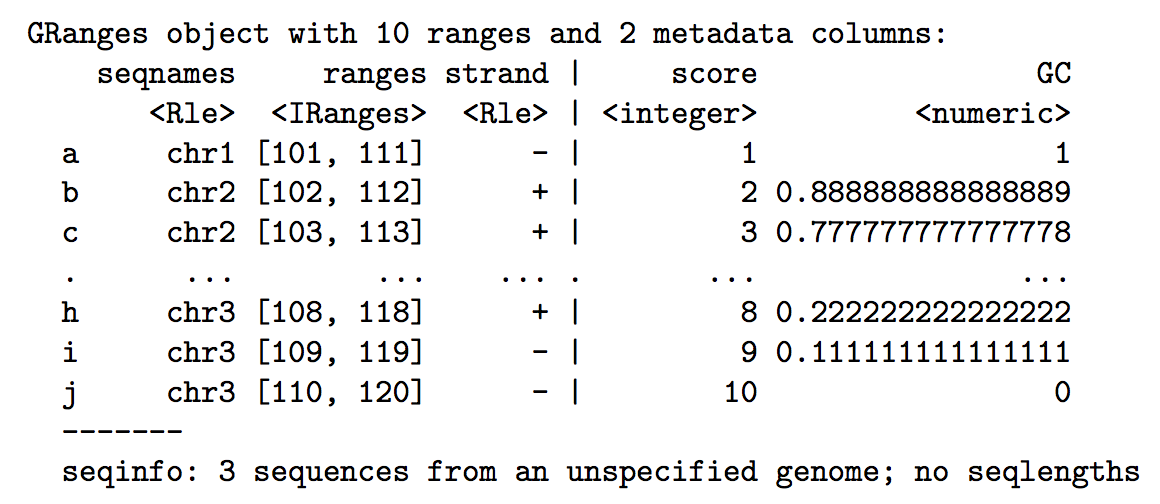
\includegraphics[width=1.0\textwidth]{images/Granges.png}
  \caption[Granges object]{\label{fig:granges} Example of Granges object.}
  \end{figure}
  \item [\sigla{SE}{SummarizedExperiment}:]  This data structure, exemplified in Figure \ref{fig:SE}, is a  matrix-like container where rows represent ranges of interest (as a GRanges object) and columns represent samples (with sample data summarized as a DataFrame). It can contains one or more assays, each represented by a matrix-like object of numeric or other mode.
  \begin{figure}[ht!]
  \centering
  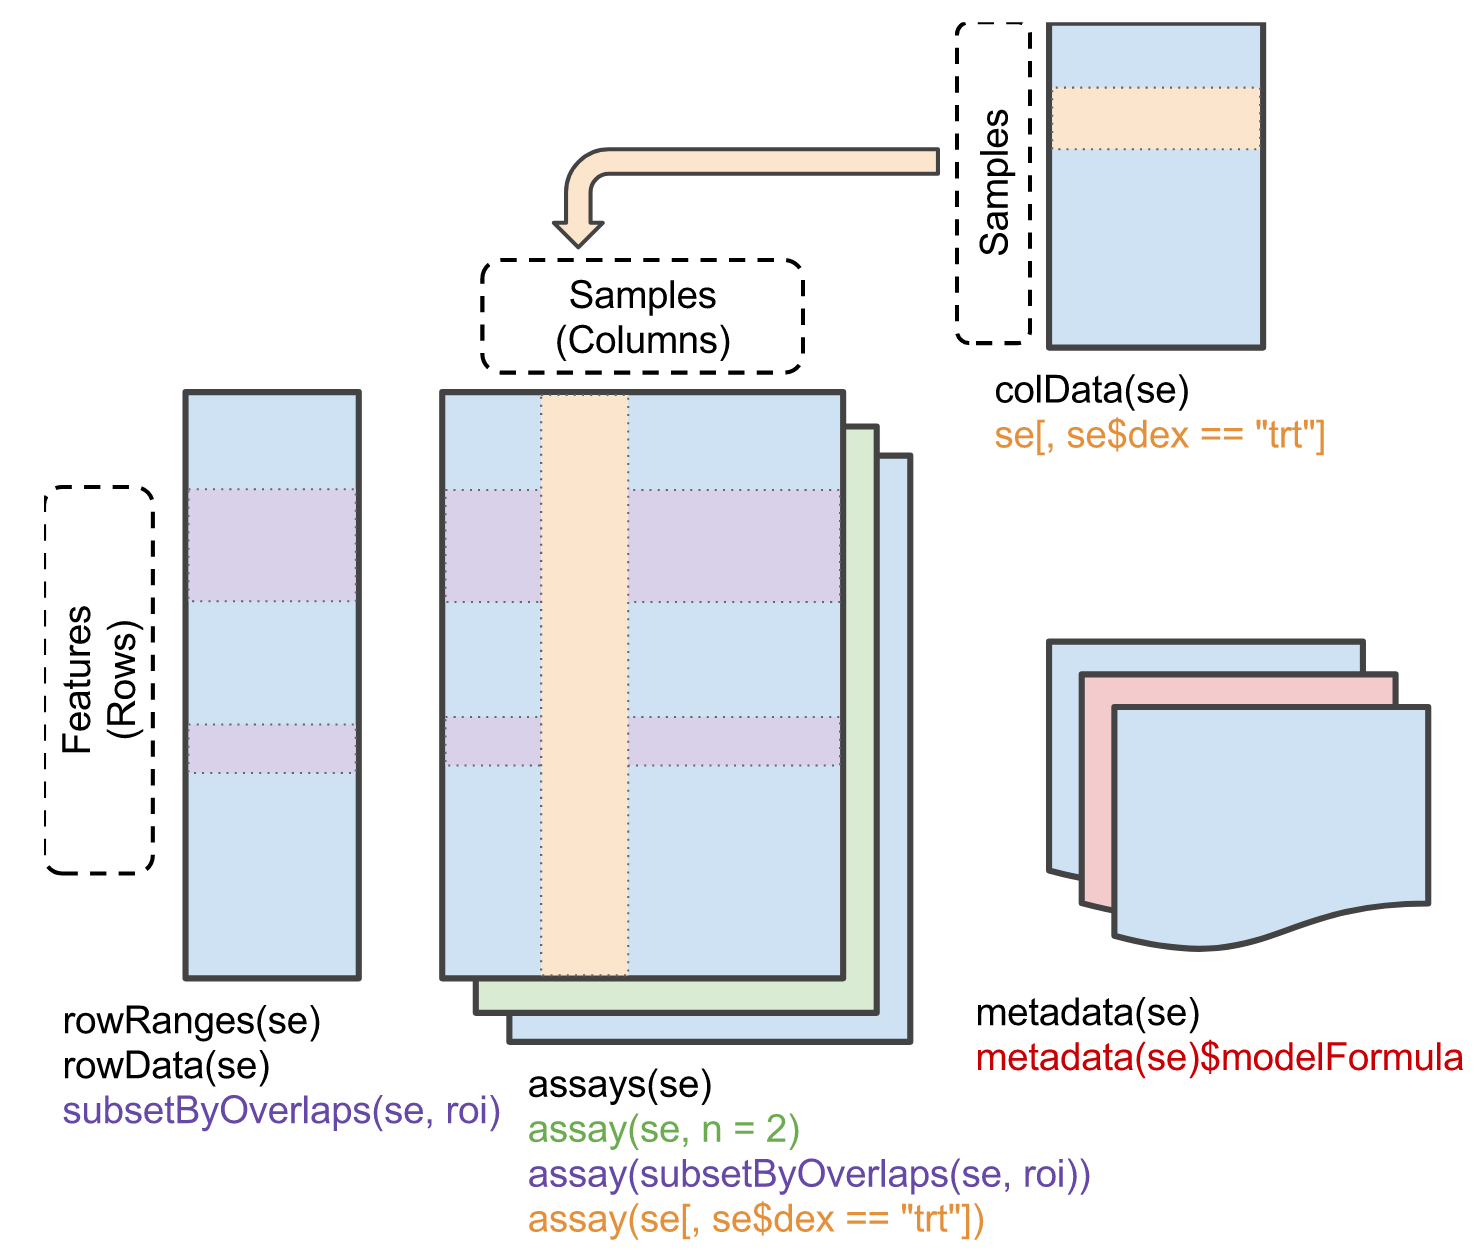
\includegraphics[width=1.0\textwidth]{images/summarizedExperiment.png}
  \caption[Sumarized Experiment object]{\label{fig:SE} Example of Sumarized Experiment object. Figure reproduced from SummarizedExperiment manual \cite{SummarizedExperiment}.}
  \end{figure}
  \item [\sigla{MAE}{MultiAssayExperiment}:] This data structure is an integrative environment where multiple assays are managed and preprocessed for genomic data analysis.  It is composed of at least two metadata matrices, one with the phenotype metadata (i.e. clinical data) and one table mapping each data column from different assays to a entry in the phenotype metadata. The data handle by this data structure can be several SummarizedExperiment objects (i.e DNA methylation, gene expression, copy number, histone modification signals).

\end{description}





\section{(Epi)Genomic data analysis} \label{sec:concept-analysis}

\subsection{Integrative analysis}
Often the onset and progression of cancerous diseases are
linked to the aberrant function of proteins and alterations in gene expression,
which has led research in genetics in search of the molecular alterations responsible for such aberrant behavior.
Among the types of alterations genetic and epigenetic
that can impact gene function are, gene copy number
(CN), DNA methylation, single nucleotide variations (SNV), and indels (small insertions and
deletions).
These variations can have a direct effect by modifying
 the function of the gene product, for example, a
indel in a coding region, or an indirect effect such as
the modification of  regulatory regions which can interfere
 with gene expression by inhibiting transcription \cite{thingholm2016strategies}.

Furthermore, recent technological developments have enabled the creation of genome-wide data for multiple types of variations.
Although individual analyzes of these variations helped  increasing knowledge of the genome and of complex
disorders, integrative analyses that evaluate cancer transcriptome data in the context of other data sources are often capable of extracting deeper biological insight from the data \cite{rhodes2005integrative}.

In this section we will highlight several integrative  approaches, including meta-analysis for extracting robust profiles from independent data sets, enrichment analysis for identifying coordinately regulated functional gene modules, protein interaction networks for detecting interaction complexes deregulated in cancer, transcriptional networks for inferring regulatory mechanisms in cancer and analyses of model system profiles with human tumor profiles for inferring activity of oncogenic pathways.

\subsubsection{Functional enrichment analysis of cancer signatures}

A \sigla{GSEA}{gene set enrichment analysis} or functional enrichment analysis is a method to identify classes of genes or proteins that are over-represented in a large set of genes or proteins and may have an association with disease phenotypes.
This type of analysis integrates  differentially expressed genes identified by a  \sigla{DEA}{differential expression analysis}  with external functional information which is necessary for interpreting and summarizing large cancer signatures.
Most approaches use external annotation databases such as Gene Ontology which is a database of controlled vocabulary gene annotations describing the biological processes, molecular functions and cellular localizations of genes as a resource for enrichment analysis in cancer signatures.

Let $L$ be a  list of genes ranked by their differential expression between the classes, the goal of GSEA is to determine whether members of a gene set $S$ tend to occur toward the top (or bottom) this list,  which might correlate with the phenotypic class distinction \cite{subramanian2005gene}.

\subsubsection{Protein interaction networks and cancer signatures}

A major objective of systems biology is to organize molecular interactions as networks \cite{vinayagam2014integrating}. \sigla{PPIs}{Protein-protein interactions} are essential to almost every process in a cell and are not only crucial for understanding cell physiology in normal and disease states, since the disruption of protein-protein interactions may result in disruption of the cell component or process to which they contribute compromising the cell viability or even leading to cell death, but also for the drug development, since drugs can affect PPIs \cite{PPIs,alzate2009neuroproteomics}.
These interactions are represented as \sigla{PPIN}{Protein-protein interaction networks}, a mathematical representation of the physical contacts between proteins in the cell.
The totality of PPIs that happen in a cell, an organism or a specific biological context is called interactome.

 A detailed human interactome network that captures the entire cellular network is invaluable in interpreting cancer signatures, allowing one to infer activated subnetworks and specific proteins that are most important to a subnetwork. For example, for a given set of overexpressed proteins in the same subnetwork, one specific protein that interacts with the entire subnetwork might be the key to control the expression the entire subnetwork.

 A lot of this information is available through molecular interaction databases such as IntAct (\burl{ http://www.ebi.ac.uk/intact}) \cite{orchard2013mintact}.

\subsubsection{Transcriptional targets and cancer signatures}

Similar to the Protein-protein interaction networks, global transcriptional networks, which defines directional pathways (i.e. which gene actives are activated by a given gene), have the potential to improve the interpretation of cancer signatures. For example, if the targets of all transcription factors  were known, then one could easily infer which transcription factors must be activated in a tumor to yield the observed cancer signature. With that information, it is possible to reduce a complex cancer signature to a small number of activated transcriptional factors which will be potential therapeutic targets.

The identification of transcription factor-binding sites (TFBSs) is done using high throughput experimental methods  such as ChIP-Chip and  \sigla{ChIP-seq}{ChIP-sequencing} which identifies a region of 100–1000
base pairs (b.p.) in which the TFBS
(typically 9-15 b.p.) resides \cite{jayaram2016evaluating}.
In-silico  sequence-based methods were developed to predicted TFBSs. These methods scan
 a DNA sequence of interest
with a \sigla{PWM}{position weight matrix},a $4 x n$ matrix of
scores for each of the 4 bases across each position in the
binding motif, for a transcription factor of interest and perform a pattern-matching.
PWM models can be obtained from a number of resources including the the open access database JASPAR \cite{portales2009jaspar}, HOCOMOCO \cite{kulakovskiy2013hocomoco} and HOMER \cite{heinz2010simple}. Among the existing  software that scans a sequence database for individual matches to each of the motifs are \sigla{FIMO}{Find Individual Motif Occurrences} \cite{grant2011fimo}, HOMER \cite{heinz2010simple} and PATSER \cite{turatsinze2008using}.

\subsubsection{Human Epigenomes}
The human body contains  more than 200 different cell types
each one has an identical copy of the genome but expresses a distinct set of genes, due to their epigenome which in each cell regulates gene expression in a number of ways - by organizing the nuclear architecture of the chromosomes, restricting or facilitating transcription factor access to DNA, and preserving a memory of past transcriptional activities \cite{rivera2013mapping}.
The integrative analysis of epigenomic maps, which references to the collection of DNA methylation state and covalent modification of histone proteins along the genome \cite{bonasio2010molecular}, has been shown to be important in the study of the gene regulatory programs \cite{gifford2013transcriptional,hawkins2010distinct,rada2012epigenomic}. Table \ref{histonemarks}
shows a summary of the epigenomic marks and their associate role.

\begin{landscape}


\bgroup
\def\arraystretch{2.0}%  1 is the default, change whatever you need
\begin{table}[]
\centering
\small
\caption[Histone and epigenomic marks]{Core set of five histone modification marks and other epigenomic marks}
\label{histonemarks}
\begin{tabular}{lp{14cm}}
\toprule
\toprule
 \textbf{Histone marks}   & \textbf{Role} \\ \toprule \toprule
 Histone H3 lysine 4 trimethylation (H3K4me3)  & Promoter regions \cite{heintzman2007distinct,bernstein2005genomic} \\
 Histone H3 lysine 4 monomethylation (H3K4me1) & Enhancer regions \cite{heintzman2007distinct}  \\
 Histone H3 lysine 36 trimethylation (H3K36me3) & Transcribed regions  \\
 Histone H3 lysine 27 trimethylation (H3K27me3) & Polycomb repression \cite{bonasio2010molecular}  \\
 Histone H3 lysine 9 trimethylation (H3K9me3) & Heterochromatin regions \cite{peters2003partitioning} \\
 Histone H3 acetylated at lysine 27 (H3K27ac)  &  Increase activation of genomic elements \cite{heintzman2009histone,rada2011unique,creyghton2010histone} \\
 Histone H3 lysine 9 acetylation  (H3K9ac)  & Transcriptional activation \cite{nishida2006histone} \\
 DNase hypersensitivity &  Regions of accessible chromatin \cite{thurman2012accessible}\\
 DNA methylation & Repressed regulatory regions \cite{cedar2009linking,moore2013dna}\\  \bottomrule
\end{tabular}
\end{table}
\egroup
\end{landscape}

Using these set of epigenetic marks, it is possible to
 discover epigenomic states which would aid in understanding
 “non-coding” genomic elements \cite{statepaintr}.
 Several tools can use those marks to infer chromatin-state such as ChromHMM \cite{ernst2012chromhmm} and StatePaintR \cite{statepaintr}.
A 15-state model created from ROADMAP data using ChromHMM is presented as follows: active TSS-proximal promoter states (TssA, TssAFlnk), a transcribed state at the 5’ and 3’ end of genes showing both promoter and enhancer signatures (TxFlnk), actively-transcribed states (Tx, TxWk), enhancer states (Enh, EnhG), and a state associated with zinc finger protein genes (ZNF/Rpts). The inactive states consist of constitutive heterochromatin (Het), bivalent regulatory states (TssBiv, BivFlnk, EnhBiv), repressed Polycomb states (ReprPC, ReprPCWk), and a quiescent state (Quies) \cite{kundaje2015integrative}.
Those precomputed chromatin-state segmentation from
 public databases such as Blueprint, ENCODE and ROADMAP using ChromHMM (\burl{http://compbio.mit.edu/ChromHMM/})
 are available at \burl{http://egg2.wustl.edu/roadmap/web_portal/chr_state_learning.html#core_15state} and
 using StatePaintR  are available at \burl{www.statehub.org}.

These data are extremely useful to characterize each different region of the genome.
For example, using those information \citeonline{kundaje2015integrative} were able to identify enhancer regions
containing strong H3K27ac signal which showed a higher DNA accessibility,
lower methylation, and higher TF binding than enhancers regions lacking H3K27ac.
Those regions with the strong H3K27ac signal are more likely to have a regulatory role.

\subsection{Statistical analysis}

\subsubsection{Hypothesis Testing}

Human genetic studies aim to identify if a phenotype is related to the genotypes
at various loci, that is, if genetic variations have an influence on the risk of
disease or other health-related phenotypes.
Statistical analysis is a crucial to present the findings in an
interpretable and objective manner \cite{sham2014statistical}.

The most popular hypothesis testing approach used to test if
genotypes and phenotypes are related  is the frequentist significance testing approach.
This is a classical approach that involves setting up two competing hypothesis: a
null hypothesis ($H_0$\simbolo{H_0}{Null hypothesis}) and an alternative hypothesis ($H_1$\simbolo{H_1}{Alternative hypothesis}).

Computing the statistical significance can be done using a one-tailed or a two-tailed test.
A two-sided test is appropriate to evaluate both directions of the test, for example,
is the estimated value smaller or higher than the reference, which actually tests if the
 estimated value is different from the reference.
A one-sided test is appropriate to evaluate only one direction of the test,
for example, is the estimated p-value smaller than the reference.
An example in genetic studies for a two-sided test would be $H_0$
hypothesis that genotypes have no effect on the phenotypes
while the $H_1$ hypothesis is that there is an effect.
Table \ref{hypothesis-tests} shows other examples.

% Please add the following required packages to your document preamble:
% \usepackage{booktabs}
\begin{table}
\centering
\caption[Hypothesis tests]{Example of three hypothesis tests about the population mean $\mu$. In genetics it could be the mean level of expression of a gene.}
\label{hypothesis-tests}
\begin{tabular}{@{}lll@{}}
\toprule
\multicolumn{1}{c}{\textbf{Type}} & \multicolumn{1}{c}{\textbf{Null}} & \multicolumn{1}{c}{\textbf{Alternative}} \\ \midrule
Right-tailed & $H_{0}:\mu = 0$ & $H_{1}: \mu >  0 $  \\
Left-tailed & $H_{0}:\mu = 0$ & $H_{1}: \mu <  0 $  \\
Two-tailed & $H_{0}:\mu = 0$ & $H_{1}: \mu \neq 0 $ \\ \bottomrule
\end{tabular}
\end{table}

\subsubsection{Making a decision: P-value approach}

The decision to reject or accept $H_0$ is made based on the calculation of a test statistic (T) from the observed data.
As the value of T depends on particular individuals in the population, repeating the study
using  different random samples from the population would provide of many different values for T.
These set of T can be summarized as a probability distribution.

% Errors in hypothesis testing
Even though, the decision made to reject or accept $H_0$ just state that we had
enough evidence to behave one way or the other.
The rejection of the null hypothesis does not prove that the alternative hypothesis is true as
the acceptance the null hypothesis does not prove that the null hypothesis is true.
It might happen that null hypothesis was rejected when it was true, or it was not
rejected when it was false. The first error in statistics is called a Type I error ("false positive"),
 while the second is called a Type II error ("false negative").
Table \ref{type_errors} shows the relations between truth/falseness of the null hypothesis and outcomes of the test.

The rate of the type I error  or significance level
$\alpha$\simbolo{\alpha}{Significance level} is the probability of having a false positive.
Normally, the significance level is set to 5\%, implying that it is acceptable to have a 5\%
probability of incorrectly rejecting the null hypothesis. With the same logic, the rate of the
type II error is denoted by $\beta$\simbolo{\beta}{rate of the type II error}.

% Please add the following required packages to your document preamble:
\begin{table}[]
  \centering
  \caption{Type I and II Errors. $\alpha = P(\textrm{Type I Error)}$, $\beta = P(\textrm{Type II Error})$}
  \label{type_errors}
  \begin{tabular}{ccc}
    \toprule
    \textbf{Decision} & \textbf{$H_0$ is True} & \textbf{$H_0$ is False} \\ \midrule
  Do Not Reject $H_0$ & Correct Decision  & Incorrect Decision (1 - $\beta$)\\
  Reject $H_0$ & Incorrect Decision (1 -  $\alpha$)& Correct Decision \\ \bottomrule
  \end{tabular}
\end{table}

To make a decision whether to reject or accept the null hypothesis, the concept of
probability value was introduced. A p-value  ($\textrm{p-value}\in [0,1]$) is the probability under a specified statistical model, constructed under a set of assumptions (normally “null hypothesis") that a statistical summary of the data
(e.g., the sample mean difference between two compared groups) would be equal to or more extreme than its observed value \cite{wasserstein2016asa}. That means, the smaller the p-value, the greater the statistical incompatibility of the data with the null hypothesis and greater the p-value more compatible is the data with the null hypothesis.
In summary, if P-value is small (e.g.$\textrm{P-value} \leq \alpha$) then the null hypothesis is rejected,
otherwise, it is not rejected.

It is important to highlight that a p-value does not measure the size of an effect or the importance of a result.
It might happen that a very small effect produces smaller p-values if the
sample size is big or measurement precision is high.
On the other hand, a large effect might produce higher p-values if
the sample size is small or measurements are imprecise.


%The P-value approach consists in the following steps to conducting any hypothesis test:
%\begin{enumerate}
%  \item Set $H_0$ (null hypotheses) and $H_1$ (alternative hypotheses)
%  \item Using the sample data and assuming the null hypothesis is true, calculate the value of the test statistic.
%  Again, to conduct the hypothesis test for the population mean $\mu$, we use the t-statistic $t^{\ast}= \frac{\bar{x}-\mu}{s/\sqrt{n}}$ which follows a t-distribution with n - 1 degrees of freedom.
%  \item Using the known distribution of the test statistic, calculate the P-value: "If the null hypothesis is true, what is the probability that we'd observe a more extreme test statistic in the direction of the alternative hypothesis than we did?"
%  \item Set the significance level, $\alpha$, the probability of making a Type I
%  error to be small - 0.01, 0.05, or 0.10. Compare the P-value to  $\alpha$.
%  If the P-value is less than (or equal to)  $\alpha$, reject the null hypothesis
%  in favor of the alternative hypothesis. If the P-value is greater than  $\alpha$,
%  do not reject the null hypothesis.
%\end{enumerate}


%For a one-sided test (for example, a test for effect size greater than zero), the definition of the P value is slightly more complicated: P* = P/2 if the observed effect
%is in the pre-specified direction, or P* = (1 – P)/2 otherwise, where P is defined as above. In the Neyman–Pearson hypothesis testing framework, if the P value is smaller than a preset threshold α (for example, 5 × 10−8 for genome-wide association studies), then H is rejected and the result is considered to be significant.

%By setting up a hypothesis test in this manner, the probability of making the error of
% rejecting H0 when it is true (that is, a type 1 error) is ensured to be α. However, another possible type of error is the failure to reject H0 when it is false (that is, type 2 error, the probability of which is denoted as β). Statistical power is defined as 1 – β (that is,
%the probability of correctly rejecting H0 when a true association is present).


\subsubsection{Correcting for multiple testing}

When performing  a set of statistical inferences simultaneously more likely erroneous inferences are to occur.
For example, if 100 tests are carried
out, then 5\% of them (that is 5 tests) are expected to
have $P-value < 0.05$ by chance when $H_0$ is, in fact, true for all the tests.
Compared to a single test (equations \ref{eq_error} and \ref{eq_error2}), the probability of having a type 1 error multiple test is given by the equations \ref{eq_multiple_error} and \ref{eq_multiple_errorb} \cite{vsidak1967rectangular}.

\begin{subequations}

\begin{align}
  P(\textrm{Making an error)} = \alpha \label{eq_error}\\
  P(\textrm{Not making an error)} = 1 - \alpha \label{eq_error2}\\
  P(\textrm{Not making an error in m tests)} = (1 - \alpha)^m  \label{eq_multiple_error}\\
  P(\textrm{Making at least 1 error in m tests}) = 1 - (1 - \alpha)^m  \label{eq_multiple_errorb}
\end{align}
\end{subequations}

To handle this multiple statistical testing problems,
some techniques  to re-calculating probabilities obtained from a statistical test which was repeated multiple times
have been developed to prevent the inflation of false positive rates.


Among the different approaches to control type I errors we have
\sigla{FWER}{Family-wise error rate} which controls the probability of at least one type I error,
and False discovery rate (FDR)
which controls the expected proportion of Type I errors
among the rejected hypotheses. Compared to FDR, controlling FWER is extremely conservative
approach as the power to detect $H_1$ gets very small.

Among the different adjustment methods to control FWER includes the Bonferroni correction
  in which the p-values are multiplied by the number of comparisons ($M * P_i < \alpha$) and the Holm correction, $P-adjusted_i = P_i * (M + 1 - i)$, where $i \in \{1,2,\dots,n\}$ and smaller the p-value is smaller will the index $i$ be \cite{aickin1996adjusting}.
 The Benjamini-Hochberg (BH) method to control FDR procedure will identify the largest $k$,
 such that $P_k \leq \frac{k}{m}\alpha$, all null hypotheses $H_i$ for $i \in \{1,\ldots,k\}$ are rejected.


These methods make the assumption that
the tests are independent tests, which often is not valid for genomics data.
For dependent tests, permutation methods are often used to calculate
 p-values.  This approach recalculates a p-value comparing
 the P-value calculated
 from the real data test with random ones,
 which are performed by randomly shuffling the case–control (or phenotype)
 labels. All $M$ tests are recalculated on the reshuffled data set, with the smallest P value of these M tests being recorded. The procedure is repeated for many times to construct an empirical frequency distribution of the smallest P values.
This  empirical adjusted P value ($P_{*}$) is given by: $$P_{*} = \frac{r + 1}{n + 1}$$ where $n$ is the number of
permutation carried out, and $r$ is the number of permuted p-values smaller than P-value calculated
from the real data.

For example, considering $\textrm{P-value = 0.1}$ and the
permuted p-values $$P_{permu} =\{0.001,0.01,0.02,0.03,0.05,0.2,0.5,0.6,1\}$$ the first 5 permuted p-values
are smaller than the original p-value, which would give us $r = 5$, resulting in:
$$P_{*} = \frac{r + 1}{n + 1} =  \frac{5 + 1}{9 + 1} = 0.6 $$
It is important to highlight that
a high number of permutations is required in order to produce reliable permuted p-value adjusted.
 \cite{davison1997bootstrap,north2002note,north2003note,sham2014statistical}.


\subsubsection{Nonparametric and parametric tests}

Statistical procedures can be classified into two groups:  Parametric and nonparametric.
Parametric statistical procedures rely on assumptions about the shape of the distribution
(i.e., assume a normal distribution) in the underlying population and about the form or
parameters (i.e., means and standard deviations) of the assumed distribution.
While nonparametric statistical procedures don't rely or rely on only a few assumptions about the shape or
parameters of the population distribution from which the sample was drawn.
Some of these procedures are summarized in Table \ref{Parametric-nonparametric}.

The most used parametric test for comparing the means of two independent groups is the t-test, which
 assumes that the data are normally distributed, that samples from different groups are independent and that the variances between the groups are equal \cite{kitchen2009nonparametric}. The most commonly used nonparametric test for indepedent samples is the  \sigla{MWU}{Mann-Whitney U-test}, which assumes that observations from the different groups are random samples (i.e. independent and identically distributed) from their respective populations, are mutually independent and are ordinal or continuous measurements. If matched or dependent samples are compared  the nonparametric  Wilcoxon signed-rank test is used \cite{whitley2002statistics}.
When there are more than two groups being compared,
the nonparametric test used is the \sigla{KW}{Kruskal-Wallis test}, a generalization of the MWU and the parametric test used is the \sigla{ANOVA}{Analysis of variance} \cite{parab2010choosing}.


\bgroup
\def\arraystretch{2.0}%  1 is the default, change whatever you need

\begin{table}[h!]
\footnotesize
\centering
\caption{Summary of parametric and nonparametric procedures.}
\label{Parametric-nonparametric}
\begin{tabular}{p{3.5cm}p{4cm}p{3cm}p{3cm}}
\toprule
\textbf{Analysis Type} & \textbf{Example} & \textbf{Parametric} & \textbf{Nonparametric} \\ \midrule
Compare means between two distinct/independent groups & Is the mean TP53 gene expression for control group different from the mean for treatment group? & Two-sample t-test & Wilcoxon ranksum test \\
Compare two quantitative measurements taken from the same individual & Was there a change in gene expression after the treatment? & Paired t-test & Wilcoxon signedrank test \\
Compare means between three or more distinct/independent groups & For a given three groups (e.g., placebo, drug \#1, drug \#2), is the TP53 gene expression different among the three groups? & Analysis of variance (ANOVA) & Kruskal-Wallis test \\
Estimate the degree of association between two quantitative variables & Is age related to the TP53 gene expression? & Pearson coefficient of correlation & Spearman’s rank correlation \\ \bottomrule
\end{tabular}
\end{table}
\egroup

It is also important to highlight that for larger sample sizes (greater than 20 or 30)
P values can be calculated using a Normal distribution,
on other words parametric tests could be used instead of the nonparametric ones \cite{vickers2005parametric}.

% https://www.ncbi.nlm.nih.gov/pmc/articles/PMC2743502/
% http://blog.minitab.com/blog/adventures-in-statistics-2/choosing-between-a-nonparametric-test-and-a-parametric-test


\subsection{Survival analysis}

In the medical sciences, in several circumstances, it is necessary to evaluate if
a treatment had a beneficial effect on the survival of patients.
For this, it is measured the fraction of patients living for a certain amount of time after treatment.

It is called "Survival times" data that measure follow-up time from a
defined starting time to the occurrence of a given event
(e.g. from the diagnosis of a disease to death) \cite{bewick2004statistics}.
These survival times are "censored" when there is a follow-up time
but the event has not yet occurred or is not known to have occurred.
That might happen if a patient drops out of the study before its end,
or if you are studying a treatment and it is not over yet.

%Standard statistical techniques cannot usually be applied
%because the underlying distribution is rarely Normal and the
%data are often ‘censored’.
\subsubsection{Kaplan–Meier method: Estimating the survival curve}

It is defined  survival function $S(t)$ is defined as the
probability of surviving at least to time t, while a
 graph of $S(t)$ against $t$ is called the survival curve.
To estimate this curve there exists the Kaplan-Meier method:
$$ S(t) = \prod_{i: t_i\leq t}\left(1 - \frac{d_i}{n_i}\right),$$
\simbolo{S(t)}{Kaplan–Meier estimator} where $d_{i}$ are the number of events and  $n_{i}$
the total individuals at risk at time $i$. Table \ref{survival-example} shows
an example of survival data and Table \ref{Kaplan-Meier-example} shows
an example of applying Kaplan-Meier method. Figure \ref{fig:survival_example}
shows a more real data example.
 It is important to highlight that
for a censored time the proportion surviving will be 1, that means
an individual is considered to be at risk of dying in the next event of the censoring
but not in subsequent events \cite{bland2004logrank}.

\begin{table}[h!]
\centering
\caption[Survival time example]{Survival time and status for a group of patients.}
\label{survival-example}
\begin{tabular}{ccc}
\hline
\multicolumn{1}{l}{\textbf{Patient ID}} & \multicolumn{1}{l}{\textbf{Survival times (in days)}} & \multicolumn{1}{l}{\textbf{Status}} \\ \hline
1 & 1 & Dead \\
2 & 1 & Dead \\
3 & 2 & Alive (censored) \\
4 & 3 & Dead \\ \hline
\end{tabular}
\end{table}

\begin{table}[h!]
\centering
\caption[Kaplan-Meier method example]{Kaplan-Meier method example for table \ref{survival-example}}
\label{Kaplan-Meier-example}
\begin{tabular}{cp{3cm}p{3cm}p{3cm}c}
\hline
\textbf{Interval} & \textbf{$n_i$: patient at risk at time $t_i^-$} &
\textbf{$d_i$ = deaths at time $t_i$} &
\textbf{$c_i$ = censored at time $t_i$} &  \textbf{$S(t)$}  \\ \hline
$[0,1)$ & 4          & 0 & 0 & 1 \\
$[1,3)$ & 4 - 0 = 4  & 2 & 1 & $1 - \frac{2}{4} = 0.5$ \\
$[3,\textrm{End of study}]$  & 4 - 2 - 1 = 1  & 1 & 0 & $0.5 * (1 - \frac{1}{1})$ = 0 \\ \hline
\end{tabular}
\end{table}


\begin{figure}
\centering
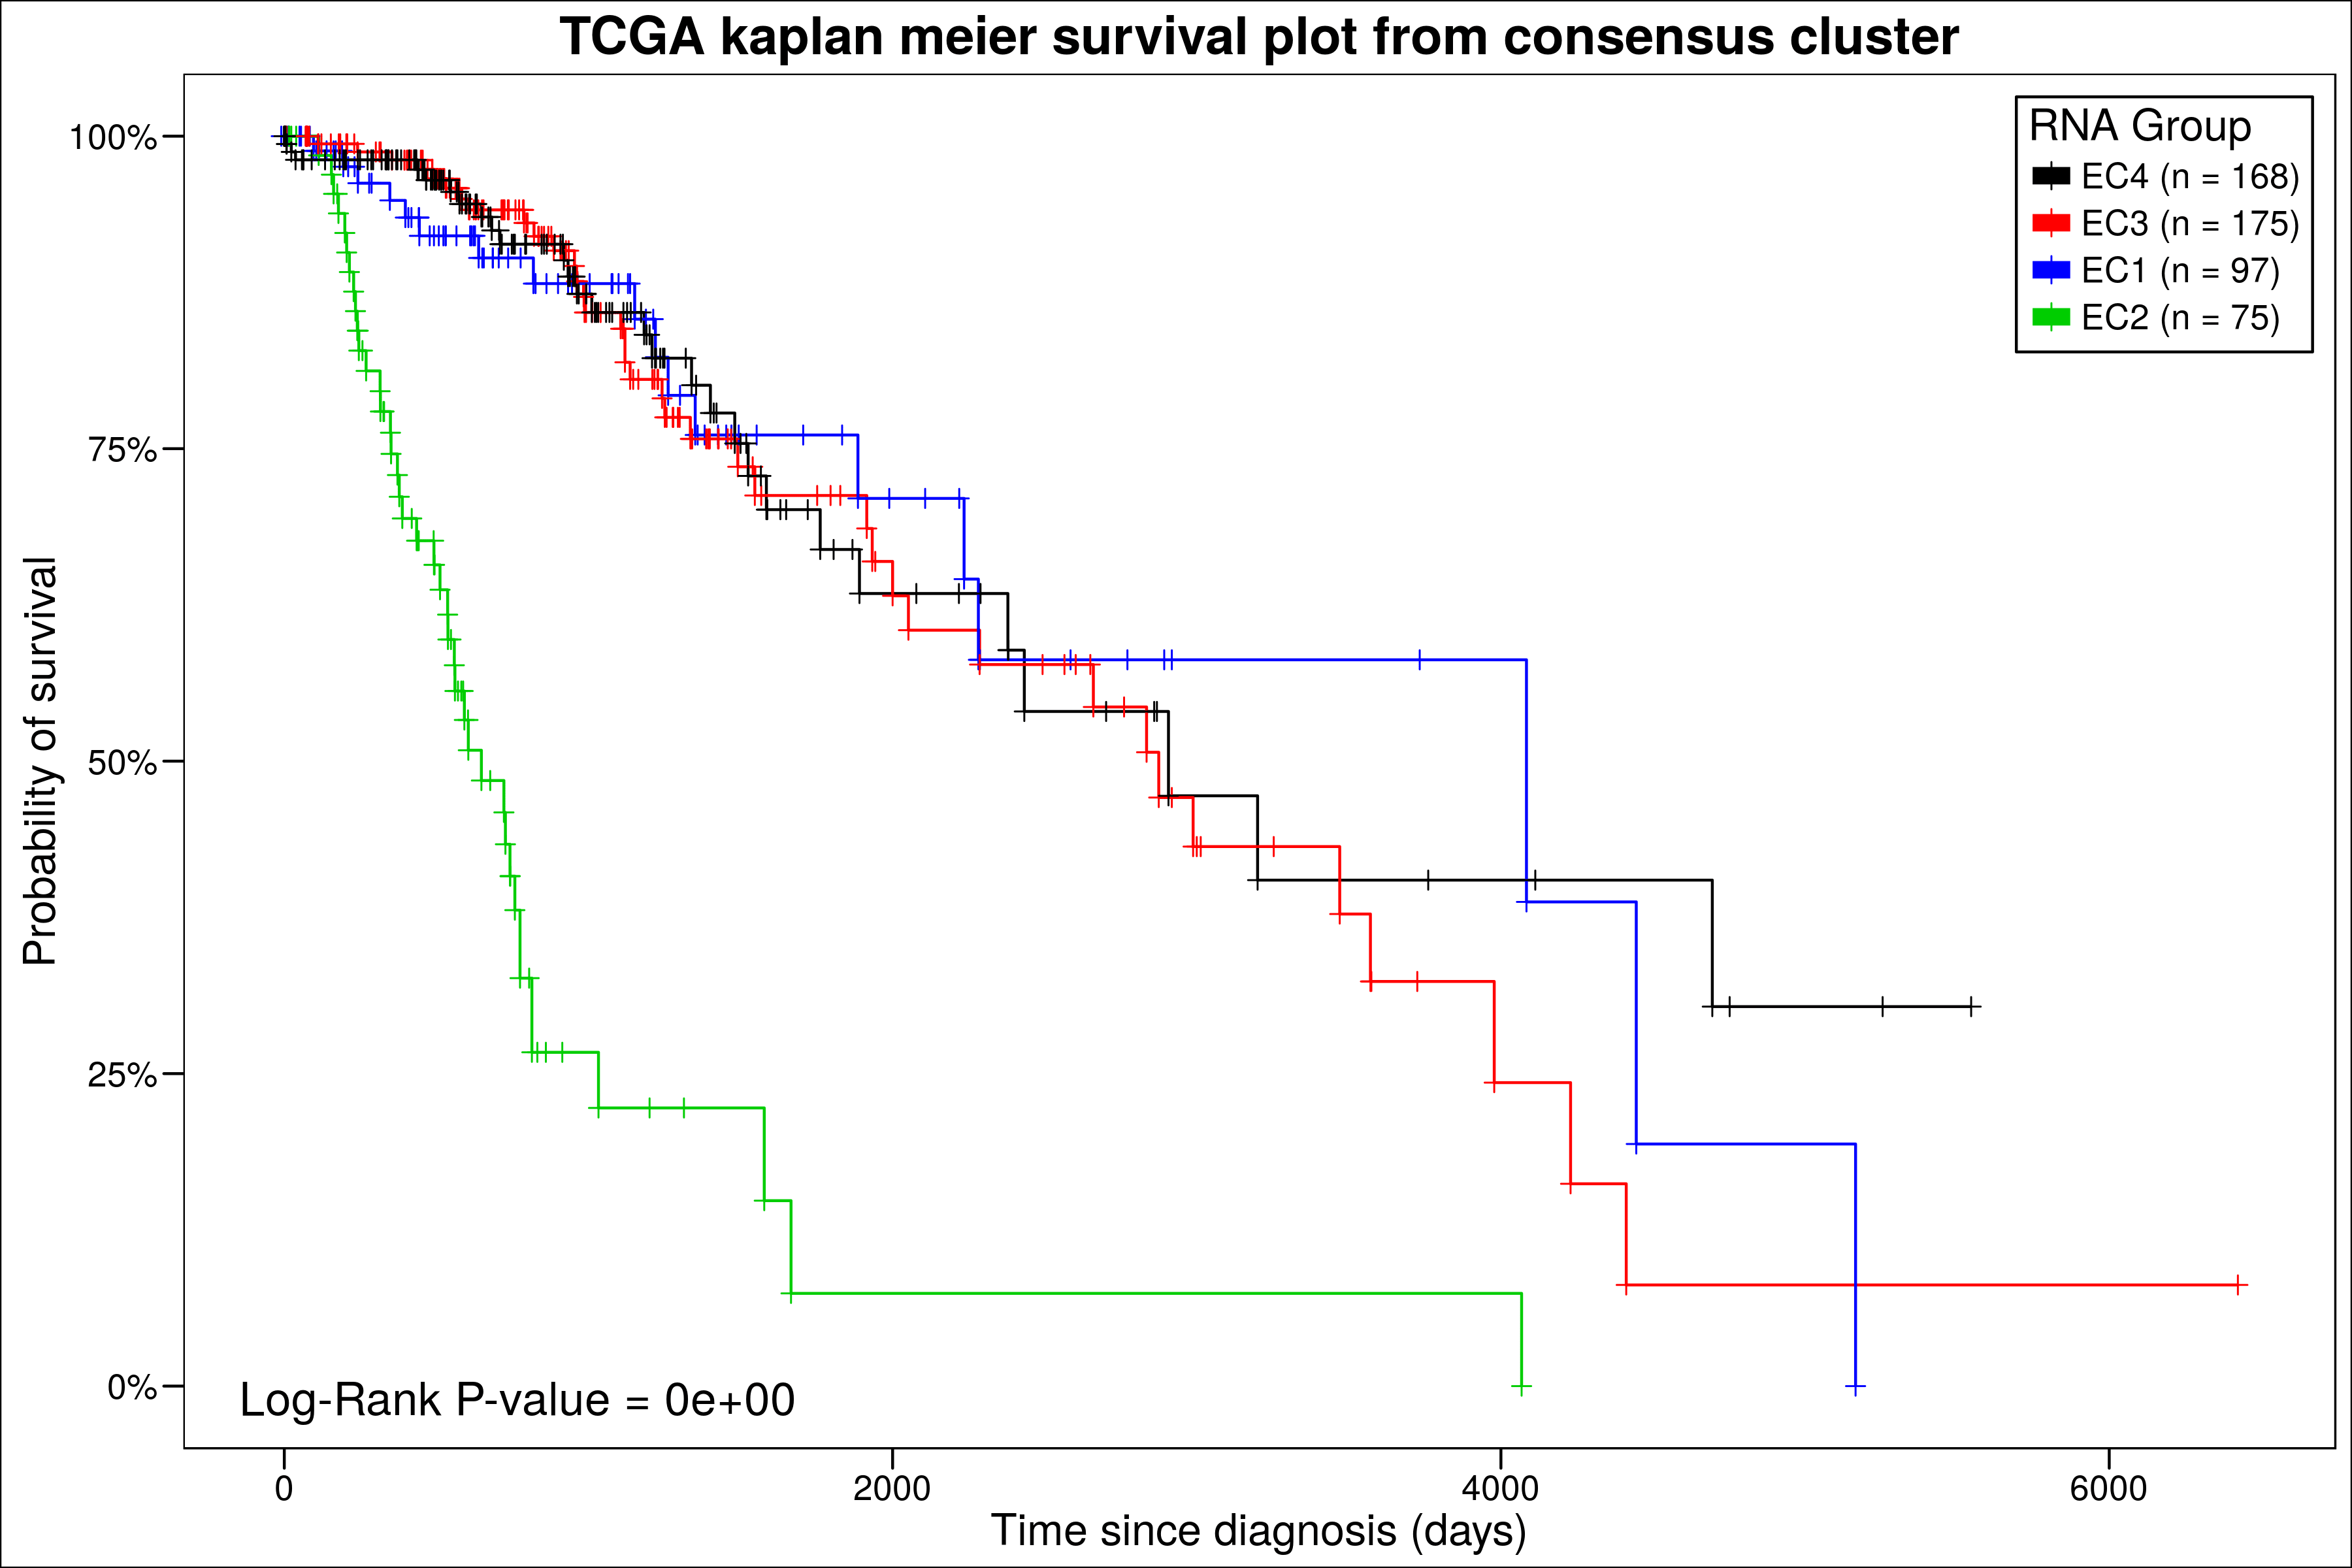
\includegraphics[width=1.0\linewidth]{images/example_survival.png}
\caption[Example of survival curve.]{\label{fig:survival_example}
Example of survival curve for TCGA samples clustered by RNA expresssion levels. Group 2 has
the worst survival. Censored data is marked (+) in the plot.}
\end{figure}



%In analyzing survival data, two functions that are dependent
%on time are of particular interest: the survival function and the
%hazard function.
%The survival function S(t) is defined as the
%probability of surviving at least to time t. The hazard function
%h(t) is the conditional probability of dying at time t having
%survived to that time.

\subsubsection{Comparing survival curves of two groups using the log-rank test}

 To compare the survival distributions of two or more groups,  the hypothesis test log-rank test is
 used to test the null hypothesis that there is no difference between the populations
 in the probability of an event at any time point.
%
 The approximated statistics used for comparison purposes for $k$ groups is
 $$T = \sum_{i \in \{1,\ldots,k\}}\frac{(O_i - E_i)^2}{E_i},$$
 where $O_i$ is the observed numbers of death in  group $i$
 while $E_i$ is its expected numbers of deaths.
 If the null hypothesis is true, $T$ is distributed approximately as a $\chi^2_{k-1}$ \cite{matthews1996using}.
If T calculated is $9.44$, and $k = 2$,  evaluating the quantile function (also known as “inverse CDF” or “ICDF”) of the chi-squared distribution the significance level of these data is equal to
$P_r(\chi^2_{1}\geq9.44) = 0.002$ \cite{yau2012r}.
For a given cut-off, normally $0.05$, the results with a p-value smaller are considered significant.

\subsection{Machine Learning}

Machine learning is a field of computer science focused on the development and application of algorithms that improve with experience \cite{mitchell1997machine}.
In genetics and genomics, it has been applied
 for the interpretation of large genomic datasets and annotation of a wide variety of genomic sequence elements.
For example, for the detection of  transcription start sites (TSSs) locations, which have proven hard to detect in silico due to the complexity and the fairly diffuse structures of Eukaryotic promoters, \citeonline{down2002computational} developed a machine-learning method is able to build useful models of promoters for more than 50\% of the human transcription start sites \cite{down2002computational}.

The machine learning techniques can be classified into two main categories: supervised and unsupervised learning \cite{mitchell1997machine}. The supervised learning, which aims to infer data labels by learning from already labeled data, has three stages: design, model, and test. The first stage refers to the selection of a learning algorithm used to learn from data (e.g. choose between support vector machines or random forest algorithms) and its training data. The second stage is the creation of a model from labeled data using the algorithm selected previously.  The last stage uses this generated model to  predict the labels of unlabeled data.
The unsupervised learning methods, on the other hand,
cluster the data without using labels, which requires an additional step in which semantics must be manually assigned to each cluster. As this discovery is not tied to previously defined classes, these methods have as benefit the ability to identify potentially novel types of genomic elements.


\subsubsection{Supervised learning}

Supervised learning is a type of machine learning algorithm that identifies patterns in data to make predictions.
Specifically, the algorithm takes a known set of input data and known responses to the data (labels) and trains a model to generate predictions for the response to new data.
The supervised learning algorithms can be classified into two categories: classification and regression.

In classification, the goal is to assign a label to an observation. That is, responses are categorical variables.
For example, given dataset known to be
an enhancer or not enhancer, one could want to predict the locations of enhancers in the genome.

In regression, the goal is to predict a continuous measurement for an observation. That is, the responses variables are real numbers. In genomics, these methods are  used in genetic epidemiology to detect association of genetic variants with a trait or disease of interest \cite{dasgupta2011brief}.




\subsubsection{Unsupervised learning}


Unsupervised learning is a type of machine learning algorithm used to draw inferences from datasets consisting of input data without labeled responses.
The most common unsupervised learning method is cluster analysis, which is used for exploratory data analysis to find hidden patterns or grouping in data. These algorithms seek to group a set of objects into clusters (groups)
such that those in the same group are more similar to each other than to those in another cluster.
The major unsupervised learning techniques used in bioinformatics are described below.
\begin{description}

\item[Hierarchical clustering:] {This clustering method builds a hierarchy of clusters,
through either a agglomerative ("bottom-up") or a divisive ("top-down") procedures.
In the agglomerative procedures, each $n$ observation starts in its own cluster and until only one cluster remains the groups with the smallest dissimilarity are merged.
On the other hand, in the divisive procedures, all observations start in one cluster and until all observations are in their own cluster the group is split into two groups with the biggest dissimilarity. To decide which clusters to merge or divide a metric to measure of dissimilarity between sets of observations is required.
Among the existing agglomerative techniques are the single linkage, also known as the nearest-neighbour technique, which defines the smallest dissimilarity between two points in each group as the dissimilarity between two groups \cite{florek1951liaison}, the complete linkage which defines the largest dissimilarity between two points in each group as the dissimilarity between two groups \cite{defays1977efficient}, the average linkage which defines the average dissimilarity overall points as the dissimilarity between two groups \cite{sokal1958statistical} and the Ward’s method which at each merge step minimizes the increase in the total within-cluster error sum of
squares, which means that  the groups leading to a minimum increase in total within-cluster variance are merged \cite{ward1963hierarchical,everitt2011hierarchical}.
The results of hierarchical clustering are usually represented in a dendrogram a branching diagram in which the objects are represented in one of the axes while the similarity between clusters are represented in the other axis by the length of the connection which joins them \cite{manning1999foundations}.}

\item[Optimization clustering techniques:]{
These are a set of non-hierarchical clustering techniques that cluster individuals into a specified number of groups, by either minimizing or maximizing some numerical criterion \cite{everitt2011hierarchical}.  One of these techniques is the k-means algorithms, which iteratively updates a partition by simultaneously relocating each object to the group to whose mean it was closest and then recalculating the group means until the groups no longer change.
More explicitly, let $S = \{S_1,S_2,\ldots,S_k\}$  be the set of $k$ clusters, this algorithm tries to minimize the squared distances of the elements from the cluster center:
$$ N(n,k) = min\sum_{g = 1}^{k}\sum_{j \in S_g}\Vert x_j - \mu_g\Vert^2,$$
where $x_j$ is a data element that belongs to a group g, and $\mu_g$ is the center of points of the $g$ group. A counterpoint of these techniques also requirement to ‘estimate’ the number of clusters in the data, for which a variety of methods
have been suggested and  most are
relatively informal and involve, essentially, plotting the value of the clustering
criterion against the number of groups in which large changes of levels in the plot are
usually taken as suggestive of a particular number of groups.
Some formal methods were also proposed such as the Silhouette index by \citeonline{rousseeuw1987silhouettes}.
And the second counterpoint of this technique is the choice of initial starting values which might lead to a local optimal solution, some solution to this problem such as a  bootstrap-like approach to ‘refine’ initial seeds are suggested \cite{steinley2003local}.
}
\item[Principal component analysis (PCA):]{
This method transforms the variables in a multivariate data set into new variables  which are uncorrelated with each other and a linear combination of the original variables. This technique provides a means of
projecting the data into a lower dimensional space, which is very useful  mainly due to the problems of high dimensional data which is called ``curse of dimensionality''.
Generally, \citeonline{verleysen2005curse} defines the curse of dimensionality as the expression of all phenomena that appear with high-dimensional data, and that have most often unfortunate consequences on the behavior and performances of learning algorithms. In summary, the number of learning data should grow exponentially with
the dimension, that means if 10 data  is reasonable to learn a 1-dimensional model, for a 2-dimensional model it will need 100 data). For example, in genetics, microarray experiments have information for thousands of genes, if each one is considered a variable we would have a thousand dimensions,
and we would need an enormous amount of observations to obtain a reliable result. If a dimensionality reduction is not performed, with a increase of data features (dimensions), it is very likely that, by chance, one feature perfectly separates the training examples into positive and negative classes, which would lead
to good performance on the training data but poor generalization to data that were not used in training \cite{libbrecht2015machine}.
}
\end{description}
